% Document class `report-template` accepts either project-plan or final-report option in
% []. This will change the title page as necessary.
%\documentclass[project-plan]{report-template}
\documentclass[final-report]{report-template}

% Packages I use in my report.
\usepackage{graphicx}
\usepackage{amsmath}
\usepackage{booktabs}
\usepackage{pgfplots}
\usepackage{pgfplotstable}
\pgfplotsset{compat=1.18}

% Directory where I saved my figures.
\graphicspath{{./figures/}}

% Metadata used for the title page - please modify.
\university{Imperial College London}
\department{Department of Earth Science and Engineering}
\course{MSc in Environmental Data Science and Machine Learning}
\title{Evaluating Physical Consistency in Video Representations Using Controlled Pendulum Simulations}
\author{Hongyi Luo}
\email{hongyi.luo25@imperial.ac.uk}
\githubusername{}
\supervisors{Dr Rossella Arcucci\\
             Dr Che Liu}
\repository{https://github.com/ese-ada-lovelace-2025/irp-hl1525}

\begin{document}

\maketitlepage  % generate title page

\section*{Abstract}
This project investigates whether pretrained vision encoders produce latent
trajectories that are sensitive to physical consistency in videos. Early
experiments with AI-generated toy videos were useful for reproducing the
evaluation pipeline, but the physical labels were not sufficiently controlled:
videos prompted to show wrong physics were often visually plausible or only
weakly wrong. To obtain a cleaner benchmark, I generated a controlled simulated
pendulum dataset containing single- and double-pendulum videos with explicitly
defined correct and wrong dynamics. Each video is sampled into frames, encoded
with multiple pretrained vision models, and analysed as a trajectory in latent
space. The main result is that wrong-physics videos tend to produce larger and
less stable frame-to-frame movements in latent space. This signal is clearer in
step-distance metrics than in straightness or curvature. DINOv2 and CLIP show
the strongest separation in the current benchmark, while MAE provides little
useful signal. These results motivate a broader analysis of latent trajectories,
patch-level feature changes, and attention maps as complementary diagnostics of
physical consistency.

\section{Introduction}
Modern video generation models can produce videos that look plausible to a
human observer, but visual plausibility does not guarantee physically consistent
motion. A generated video may show an object moving smoothly while still
violating basic physical expectations such as gravity, energy conservation, or
stable pendulum dynamics. This creates a need for evaluation tools that examine
physical consistency rather than only perceptual realism.

This report explores a representation-based approach to this problem. Instead
of directly estimating physical quantities from pixels, the method treats a
video as a temporal trajectory through the latent space of a pretrained vision
encoder. If the visual dynamics are coherent, consecutive frame embeddings
should evolve in a relatively stable way. If the video contains an injected
physical inconsistency, the latent trajectory may exhibit larger jumps or more
irregular temporal movement.

The project began with AI-generated videos of simple physical scenes. These
videos were useful for building and debugging the pipeline, but they also
revealed an important limitation: prompt-generated ``wrong physics'' examples
are not reliable ground truth. The video model may ignore the prompt, produce a
different kind of error, or make both the correct and wrong examples physically
ambiguous. The main experimental focus therefore moved to controlled simulated
videos, where the motion equations and wrong-physics interventions are defined
explicitly.

\section{Research Questions}
The current work is organised around three questions:

\begin{enumerate}
    \item Do physically wrong videos produce measurably different latent
    trajectories from physically correct videos when visual style is controlled?
    \item Which trajectory metrics are most informative: straightness,
    curvature, or frame-to-frame step-distance statistics?
    \item How do different encoder families and model scales respond to the
    same controlled physical violations?
\end{enumerate}

In addition to these quantitative questions, the project also asks whether
patch-level feature maps and attention maps can explain where the encoder is
responding. This matters because a scalar trajectory metric can indicate a
difference without showing whether the model is attending to the physically
relevant objects, such as the pendulum bob, rod, or pivot.

\section{Dataset}
\subsection{Preliminary AI-Generated Videos}
The first toy dataset contained prompt-generated videos of simple physical
scenes, including pendulum motion, free fall, frictional sliding, rolling down a
slope, and elastic collision. A second set attempted to create wrong-physics
variants. These videos allowed the baseline evaluation code to be reproduced
and tested across multiple encoders, but the examples were not sufficiently
controlled. In several cases, the wrong-physics video was only weakly wrong, or
the visual generation introduced unrelated artefacts.

\subsection{Controlled Simulated Pendulum Videos}
To address this limitation, I generated a controlled simulated dataset with
single- and double-pendulum videos. Each video has fixed visual style,
resolution, frame rate, and duration. The dataset contains correct examples
under normal gravity and damping, plus wrong examples where the dynamics are
manually altered. The current larger simulated set contains 48 videos: 12 correct single-pendulum
videos, 12 wrong single-pendulum videos, 12 correct double-pendulum videos, and
12 wrong double-pendulum videos. The wrong-physics interventions include energy
gain, gravity reversal after the middle of the video, zero-gravity segments,
overdamping, midpoint impulses, and periodic velocity kicks. Unlike the
AI-generated videos, these labels are controlled by construction. This makes the
simulated dataset a better benchmark for testing whether the evaluation pipeline
is stable and whether latent trajectories respond to physical inconsistency.

\section{Methods}
\subsection{Latent Trajectory Extraction}
Each video is uniformly sampled into $T=16$ frames. A pretrained vision encoder
maps every frame to an embedding vector $z_t$, giving a discrete trajectory
$\{z_t\}_{t=1}^{T}$ in latent space. I evaluate nine encoders covering multiple
model families:

\begin{itemize}
    \item DINOv2-small, DINOv2-base, and DINOv2-large;
    \item CLIP ViT-B/32 and CLIP ViT-L/14;
    \item SigLIP ViT-B/16;
    \item ViT-B, Swin-B, and MAE-B.
\end{itemize}

For CLIP and SigLIP, image features are extracted through the model's image
feature path. For DINOv2, ViT, Swin, and MAE-style models, frame embeddings are
obtained from the pooled output or the class token of the final hidden state.

\subsection{Trajectory Metrics}
The first metric is trajectory straightness:

\begin{equation}
    \mathrm{straightness}
    =
    \frac{\lVert z_T - z_1 \rVert_2}
    {\sum_{t=1}^{T-1} \lVert z_{t+1} - z_t \rVert_2}.
\end{equation}

A value near one means the trajectory moves almost directly from the first to
the last embedding. A lower value means the trajectory bends, loops, or
backtracks. However, for periodic motion such as a pendulum, low straightness is
not necessarily evidence of incorrect physics.

The second metric is a curvature proxy based on changes between consecutive
latent step directions:

\begin{equation}
    \mathrm{curvature}_t
    =
    1 -
    \cos \left(z_{t+1} - z_t,\ z_{t+2} - z_{t+1}\right).
\end{equation}

The third group of metrics measures frame-to-frame step distances:

\begin{equation}
    d_t = \lVert z_{t+1} - z_t \rVert_2.
\end{equation}

I report the mean and standard deviation of $d_t$. These metrics capture how
large and how variable the latent movement is over time. They are especially
relevant for the controlled pendulum videos because several wrong-physics
interventions create sudden or unstable motion.

\subsection{Feature And Attention Analysis}
The quantitative trajectory metrics are complemented by a qualitative
inspection pipeline. For selected videos, the encoder is re-run with hidden
states and attention outputs enabled. Patch tokens from the final hidden layer
are reshaped into a spatial grid, and the norm of the frame-to-frame patch
feature difference is visualised as a heatmap over the video frame. When the
model exposes attention weights, the class-token attention to patch tokens is
also overlaid on the frame.

This analysis is intended to answer a different question from the scalar
metrics: whether the representation changes are concentrated on physically
relevant regions, such as the pendulum bob, rod, and pivot, or whether the
encoder responds mainly to irrelevant background changes.

\section{Results}
\subsection{Preliminary AI-Generated Video Evaluation}
The AI-generated toy videos were useful for reproducing the evaluation workflow
and testing multiple encoders. However, the results were difficult to interpret
because the physical correctness of the videos was not controlled. Some
wrong-physics prompts produced videos that were visually smooth or only weakly
wrong. As a result, these experiments are treated as preliminary pipeline
validation rather than the main evidence. The controlled simulated pendulum
benchmark below is therefore used as the main experimental result.

\subsection{Controlled Simulated Pendulum Evaluation}
The simulated pendulum benchmark contains 48 videos and was evaluated with nine
encoders, producing 432 successful evaluation rows. Tables
\ref{tab:sim-encoder-deltas}--\ref{tab:sim-scene-deltas} summarize the main
quantitative results.

\begin{table}[t]
\centering
\caption{Wrong-minus-correct changes on the controlled simulated pendulum benchmark. Positive step-distance deltas indicate that wrong-physics videos produce larger frame-to-frame movement in latent space.}
\label{tab:sim-encoder-deltas}
\small
\begin{tabular}{lrrrr}
\toprule
Encoder & $\Delta$ straight. & $\Delta$ curv. & $\Delta$ std step & $\Delta$ mean step \\
\midrule
CLIP-B/32 & +0.017 & -0.058 & +0.546 & +0.638 \\
CLIP-L/14 & +0.032 & -0.051 & +0.658 & +0.931 \\
DINOv2-B & +0.025 & -0.042 & +3.468 & +4.527 \\
DINOv2-L & +0.026 & -0.069 & +3.649 & +4.478 \\
DINOv2-S & +0.025 & -0.038 & +3.793 & +4.491 \\
MAE-B & +0.006 & +0.010 & +0.024 & +0.030 \\
SigLIP-B & +0.017 & -0.060 & +0.492 & +0.713 \\
Swin-B & +0.011 & -0.027 & +0.998 & +1.447 \\
ViT-B & +0.018 & -0.073 & +0.702 & +0.554 \\
\bottomrule
\end{tabular}
\end{table}

\begin{table}[t]
\centering
\caption{Encoder-wise AUC when treating larger metric values as more likely to indicate wrong physics. Step-distance metrics are more reliable than straightness or curvature.}
\label{tab:sim-auc}
\small
\begin{tabular}{lrrrr}
\toprule
Encoder & straight. & mean curv. & std step & mean step \\
\midrule
CLIP-B/32 & 0.691 & 0.309 & 0.870 & 0.785 \\
CLIP-L/14 & 0.849 & 0.349 & 0.804 & 0.710 \\
DINOv2-B & 0.719 & 0.394 & 0.826 & 0.802 \\
DINOv2-L & 0.753 & 0.302 & 0.825 & 0.738 \\
DINOv2-S & 0.722 & 0.361 & 0.858 & 0.769 \\
MAE-B & 0.578 & 0.550 & 0.637 & 0.592 \\
SigLIP-B & 0.708 & 0.325 & 0.809 & 0.750 \\
Swin-B & 0.585 & 0.436 & 0.759 & 0.694 \\
ViT-B & 0.743 & 0.200 & 0.882 & 0.707 \\
\bottomrule
\end{tabular}
\end{table}

\begin{table}[t]
\centering
\caption{Scene-level wrong-minus-correct deltas pooled across encoders. Both single- and double-pendulum wrong videos increase latent step-distance metrics.}
\label{tab:sim-scene-deltas}
\small
\begin{tabular}{lrrrr}
\toprule
Scene & $\Delta$ straight. & $\Delta$ curv. & $\Delta$ std step & $\Delta$ mean step \\
\midrule
Double pendulum & +0.015 & -0.033 & +1.732 & +2.055 \\
Single pendulum & +0.024 & -0.058 & +1.453 & +1.902 \\
\bottomrule
\end{tabular}
\end{table}


The strongest and most consistent signal is in the step-distance metrics. Most
encoders show positive wrong-minus-correct deltas for both mean step distance
and step-distance variability. This means that physically wrong videos tend to
produce larger and less stable frame-to-frame movements in latent space. In
contrast, straightness and curvature are less reliable. This is expected for
pendulum motion, where a physically correct periodic trajectory does not have to
be globally straight.

To test whether this effect is larger than ordinary variation between valid
simulations, I also compute pairwise latent trajectory distances within each
encoder and scene. Correct-correct pairs provide a baseline for variation across
different initial conditions, while correct-wrong pairs test whether the
injected violations move the representation further away. This pairwise
analysis is important because it avoids relying only on absolute metric values:
it asks whether wrong physics is more different from correct physics than two
correct simulations are from each other.

The wrong-physics type breakdown further shows that not all violations are
equally visible to the encoders. Abrupt interventions such as periodic velocity
kicks and gravity changes produce stronger step-distance responses than smoother
energy-gain variants. This suggests that the current latent metrics are most
sensitive to temporal instability and sudden dynamical changes, rather than to
all forms of physical implausibility equally.

\begin{figure}[t]
\centering
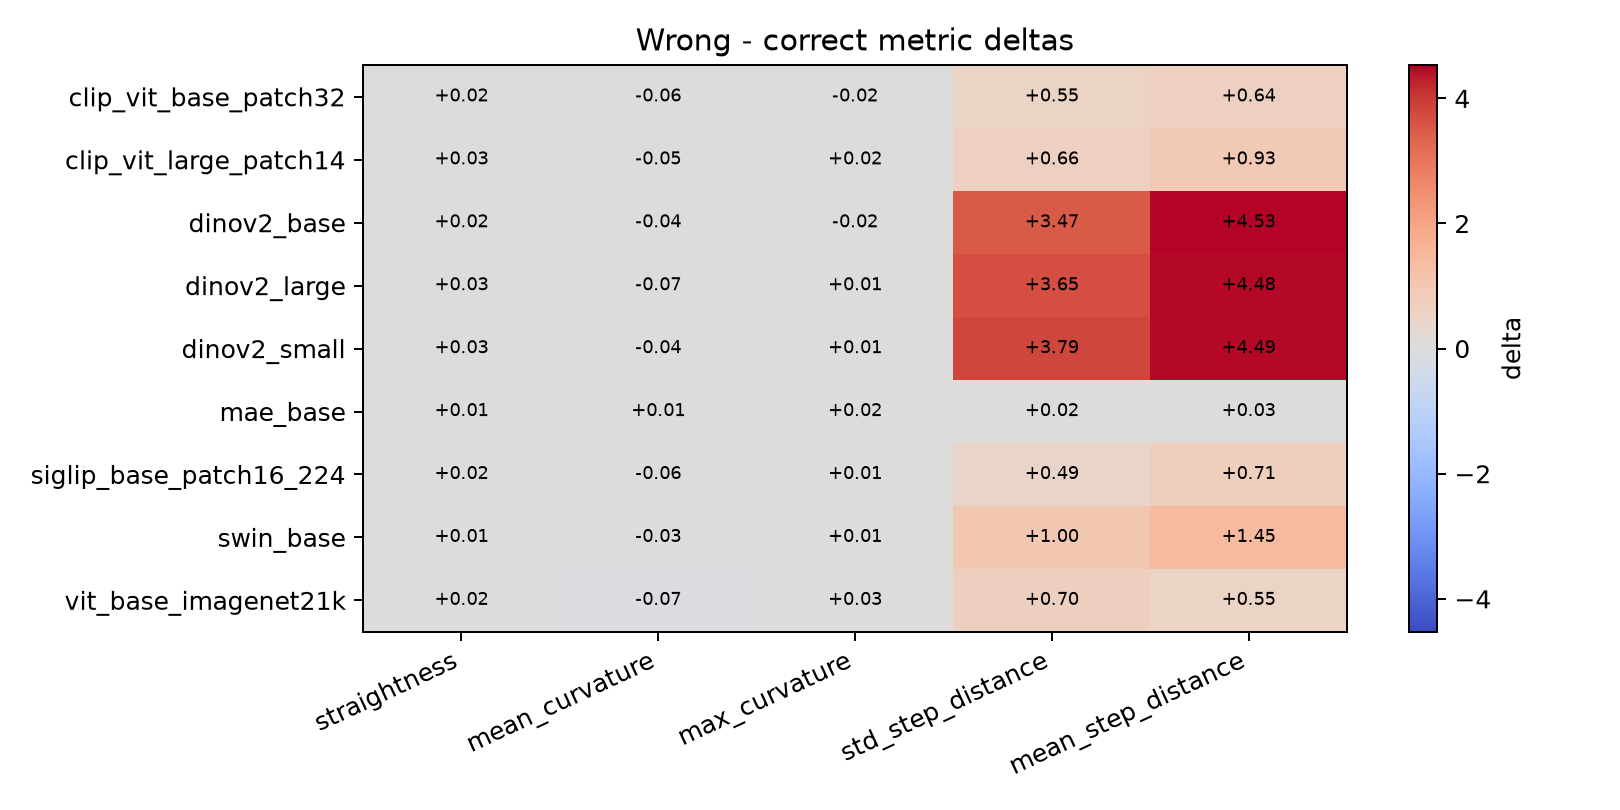
\includegraphics[width=\linewidth]{generated/simulated_pendulum/figures/delta_heatmap.png}
\caption{Wrong-minus-correct metric deltas across encoders on the simulated pendulum benchmark. The step-distance metrics show the most consistent positive changes for wrong-physics videos, while straightness and curvature are less stable.}
\label{fig:sim-delta-heatmap}
\end{figure}

\begin{figure}[t]
\centering
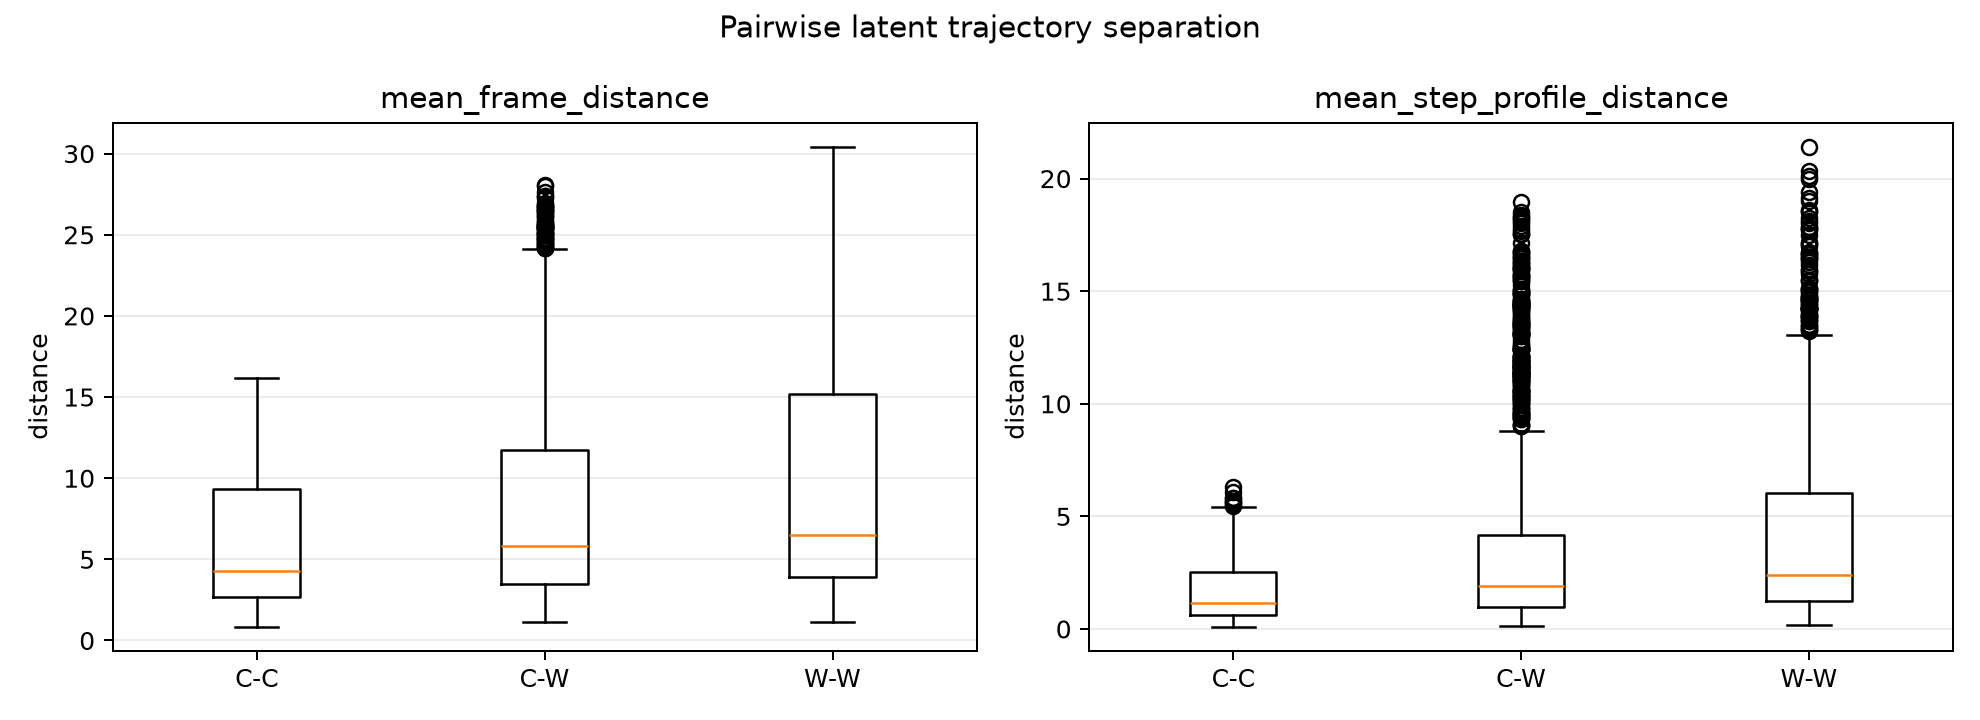
\includegraphics[width=\linewidth]{generated/simulated_pendulum/figures/pairwise_separation.png}
\caption{Pairwise latent trajectory separation. Correct-wrong pairs are compared against correct-correct pairs to test whether physical violations exceed normal variation between simulated correct videos.}
\label{fig:sim-pairwise-separation}
\end{figure}

\begin{figure}[t]
\centering
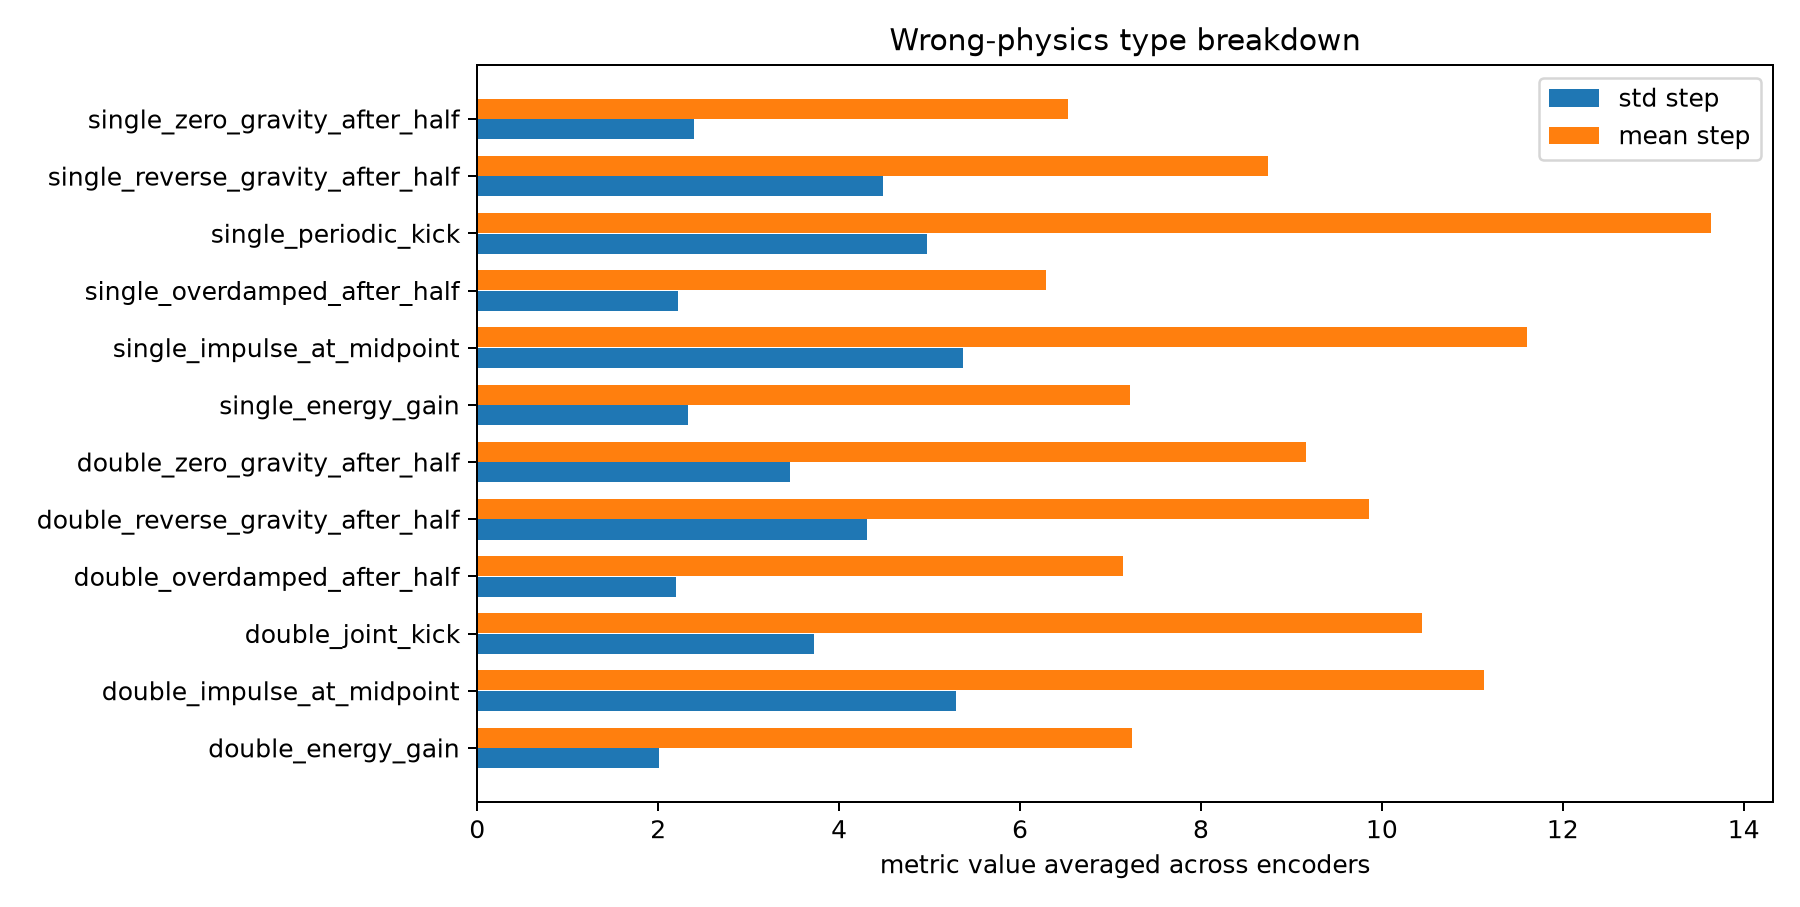
\includegraphics[width=\linewidth]{generated/simulated_pendulum/figures/wrong_type_step_distance.png}
\caption{Wrong-physics type breakdown. Abrupt interventions such as velocity kicks and gravity changes produce stronger latent movement than smoother perturbations.}
\label{fig:sim-wrong-type-breakdown}
\end{figure}

\begin{figure}[t]
\centering
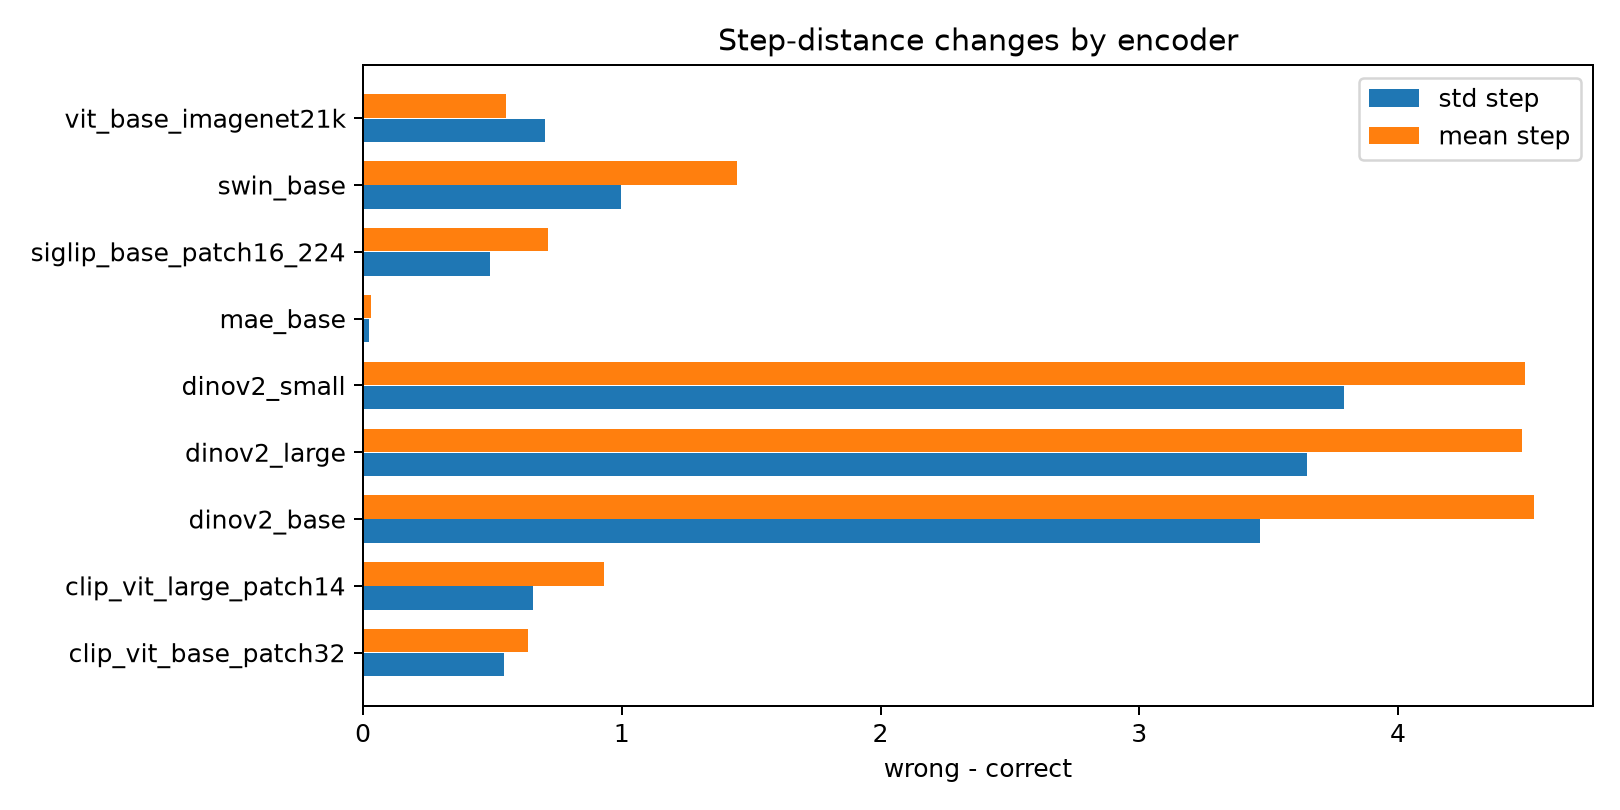
\includegraphics[width=\linewidth]{generated/simulated_pendulum/figures/encoder_step_deltas.png}
\caption{Encoder-wise changes in mean and standard deviation of frame-to-frame latent step distances. DINOv2 encoders show the largest absolute step-distance changes, while MAE does not separate correct and wrong physics in this setting.}
\label{fig:sim-encoder-step-deltas}
\end{figure}

\begin{figure}[t]
\centering
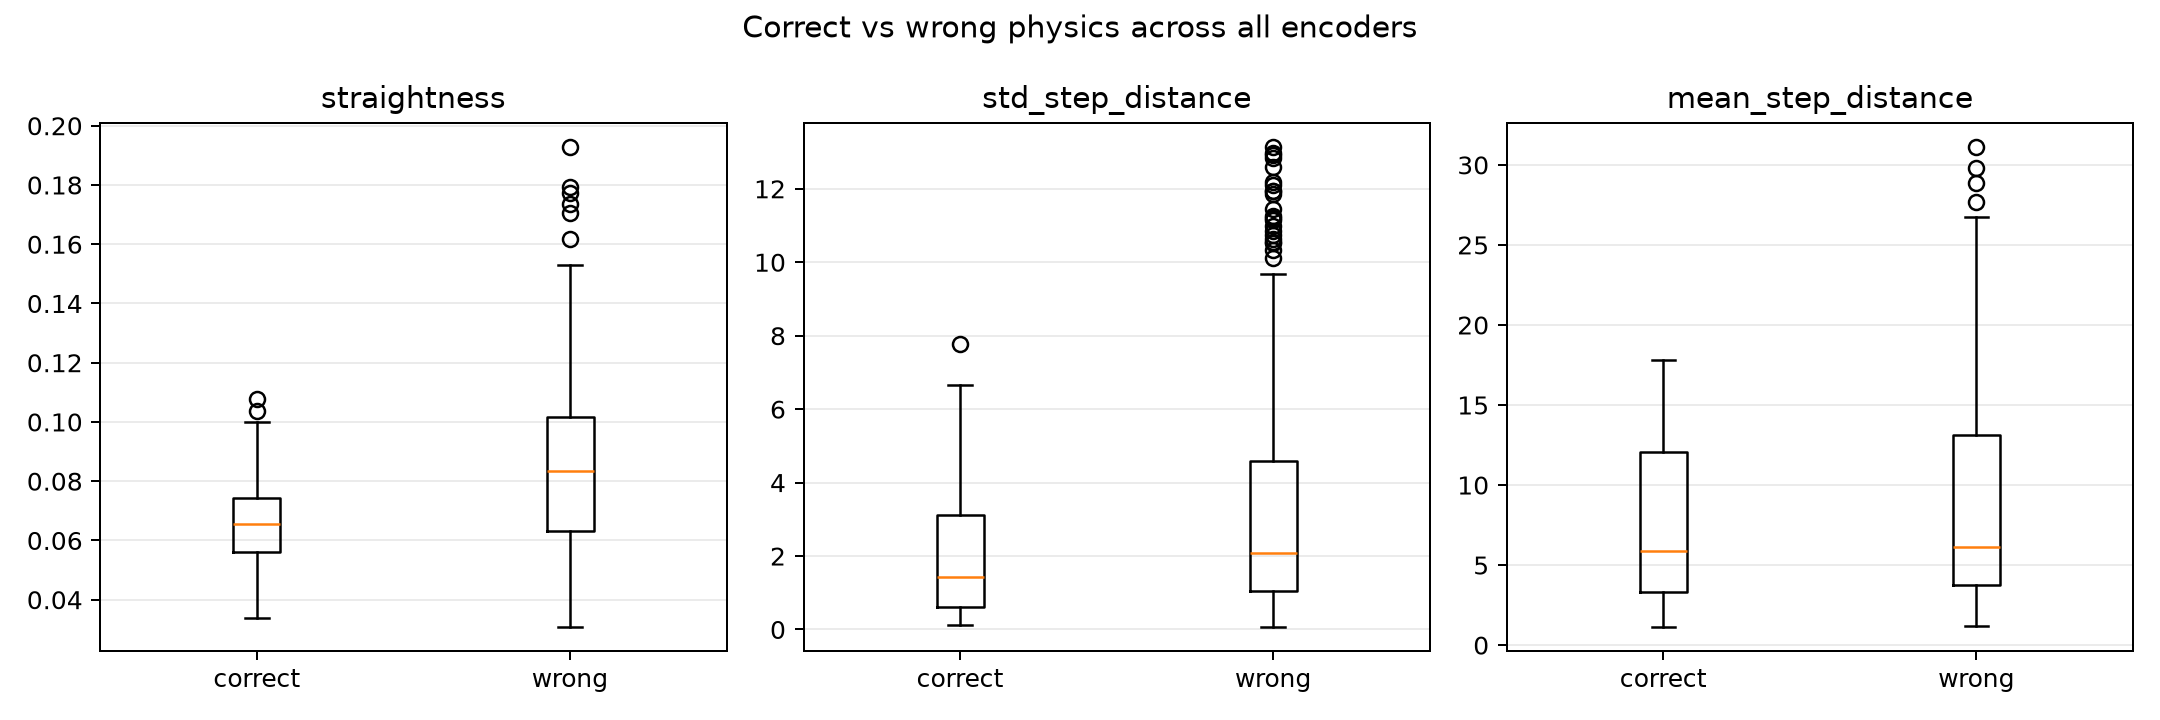
\includegraphics[width=\linewidth]{generated/simulated_pendulum/figures/metric_boxplots.png}
\caption{Correct versus wrong metric distributions pooled across encoders. Straightness overlaps strongly between the two classes, whereas wrong-physics videos produce a heavier upper tail for step-distance variability.}
\label{fig:sim-metric-boxplots}
\end{figure}

\begin{figure}[t]
\centering
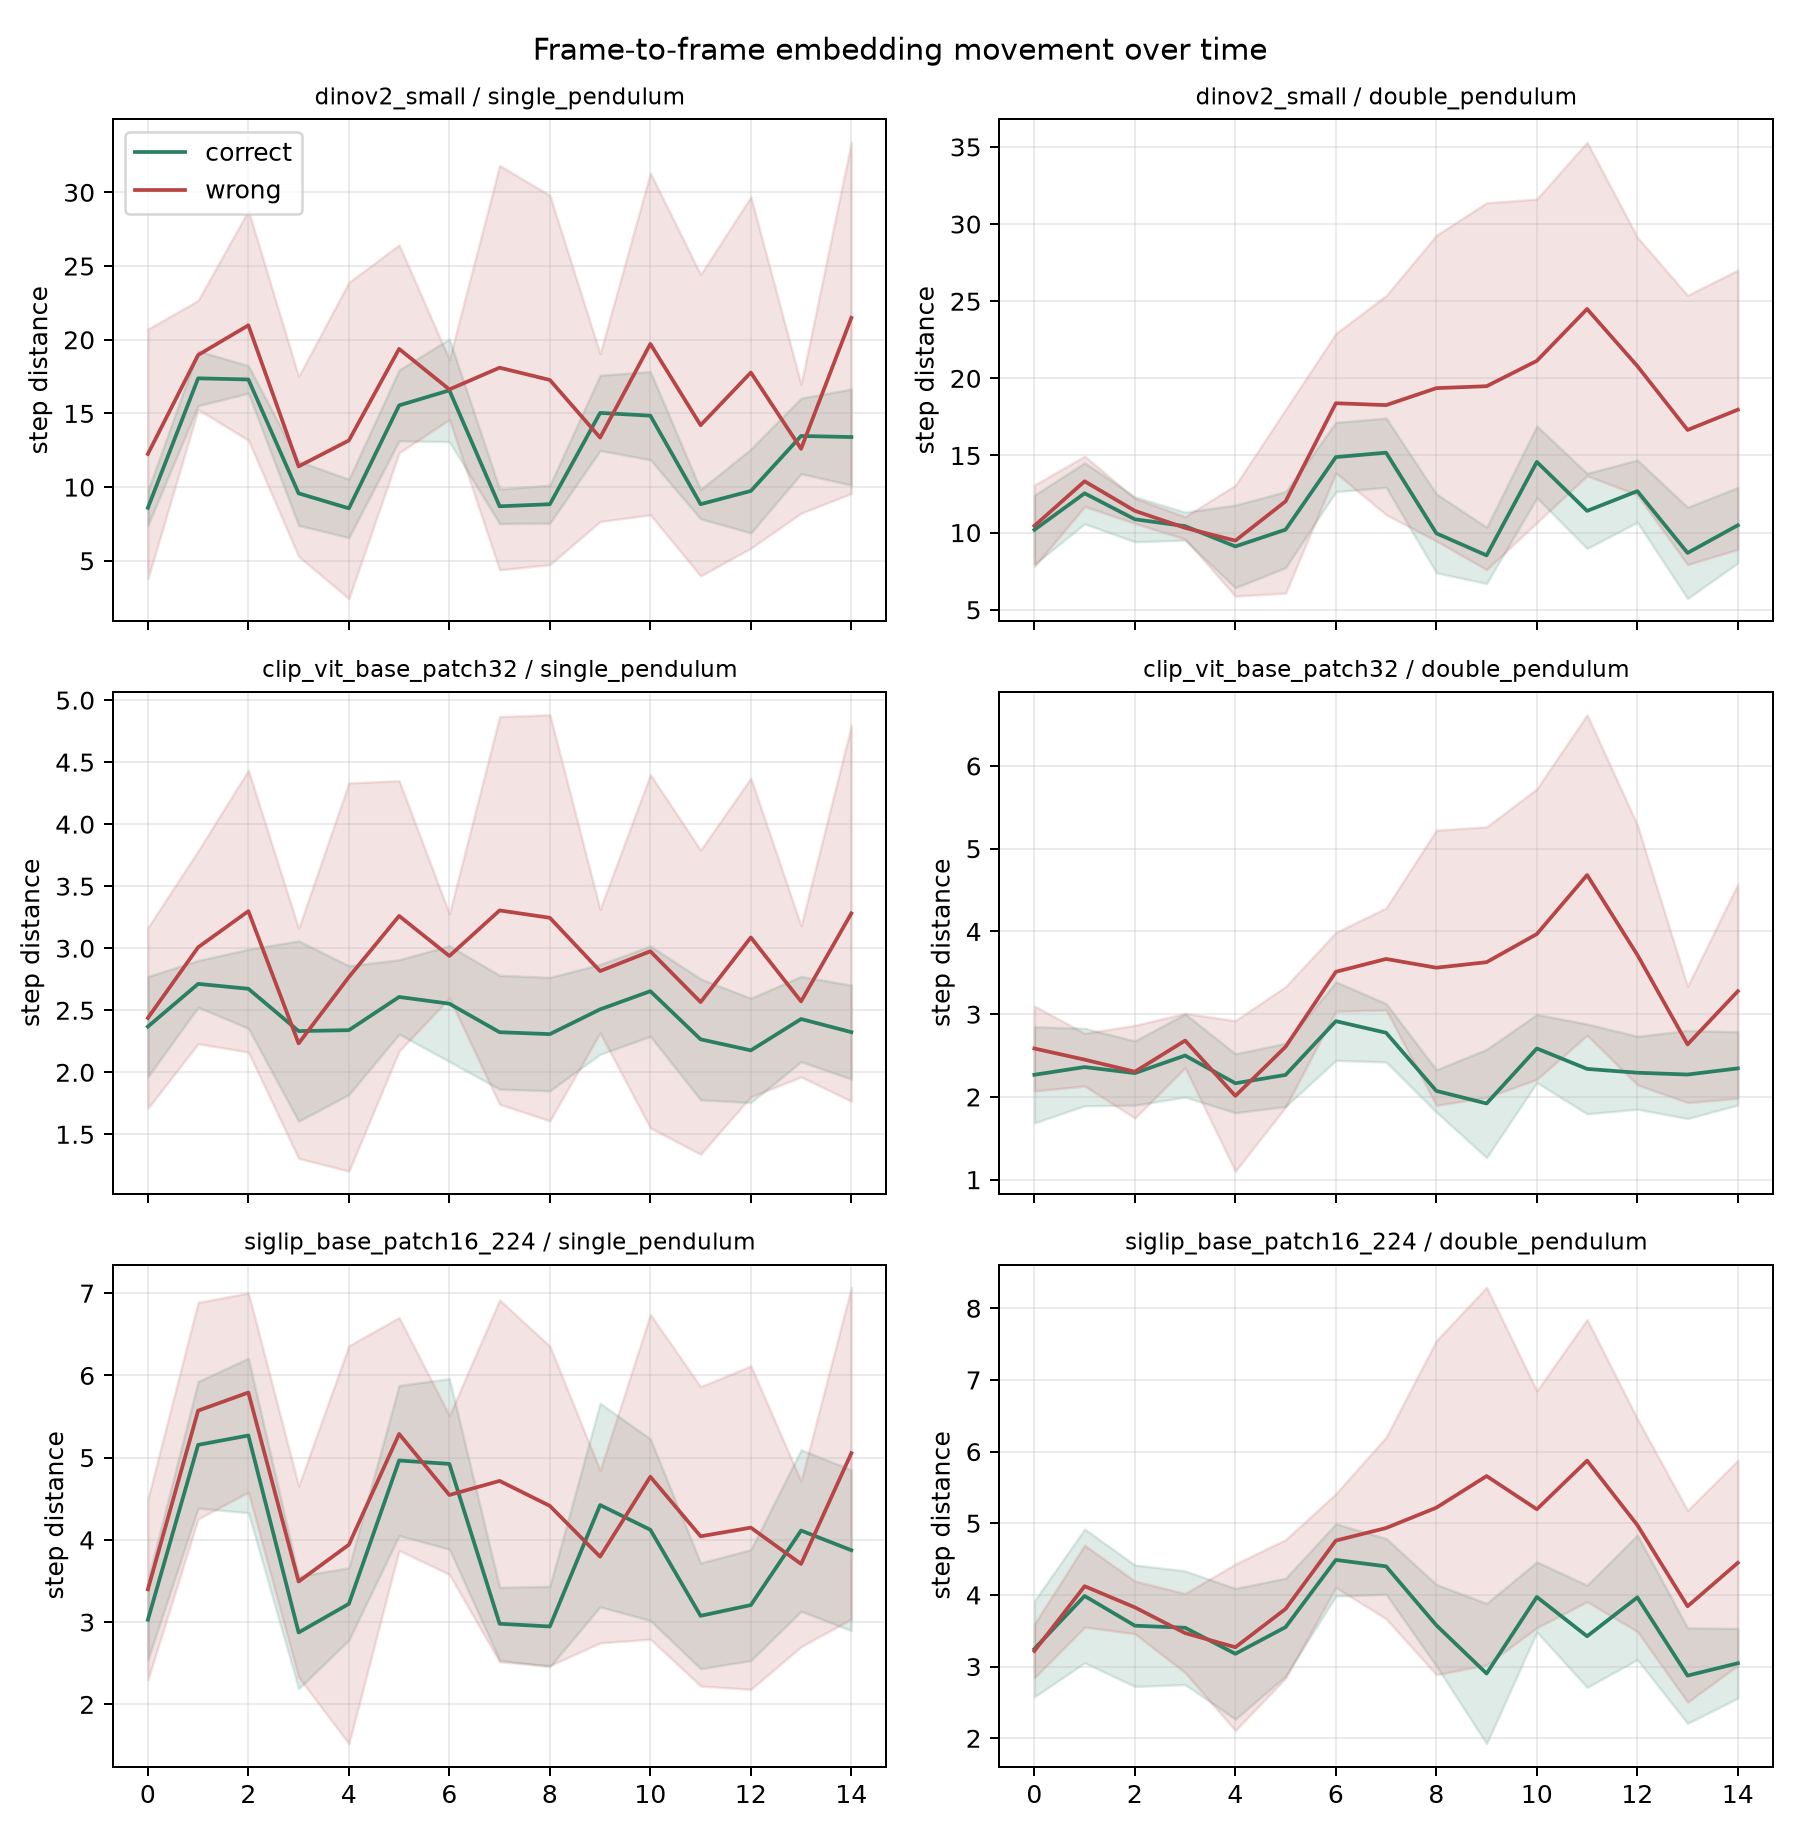
\includegraphics[width=\linewidth]{generated/simulated_pendulum/figures/step_distance_timeseries.png}
\caption{Temporal profile of frame-to-frame latent movement for representative encoders. Wrong-physics videos tend to have larger movements and occasional spikes, especially for DINOv2-small and CLIP-B/32.}
\label{fig:sim-step-timeseries}
\end{figure}

\begin{figure}[t]
\centering
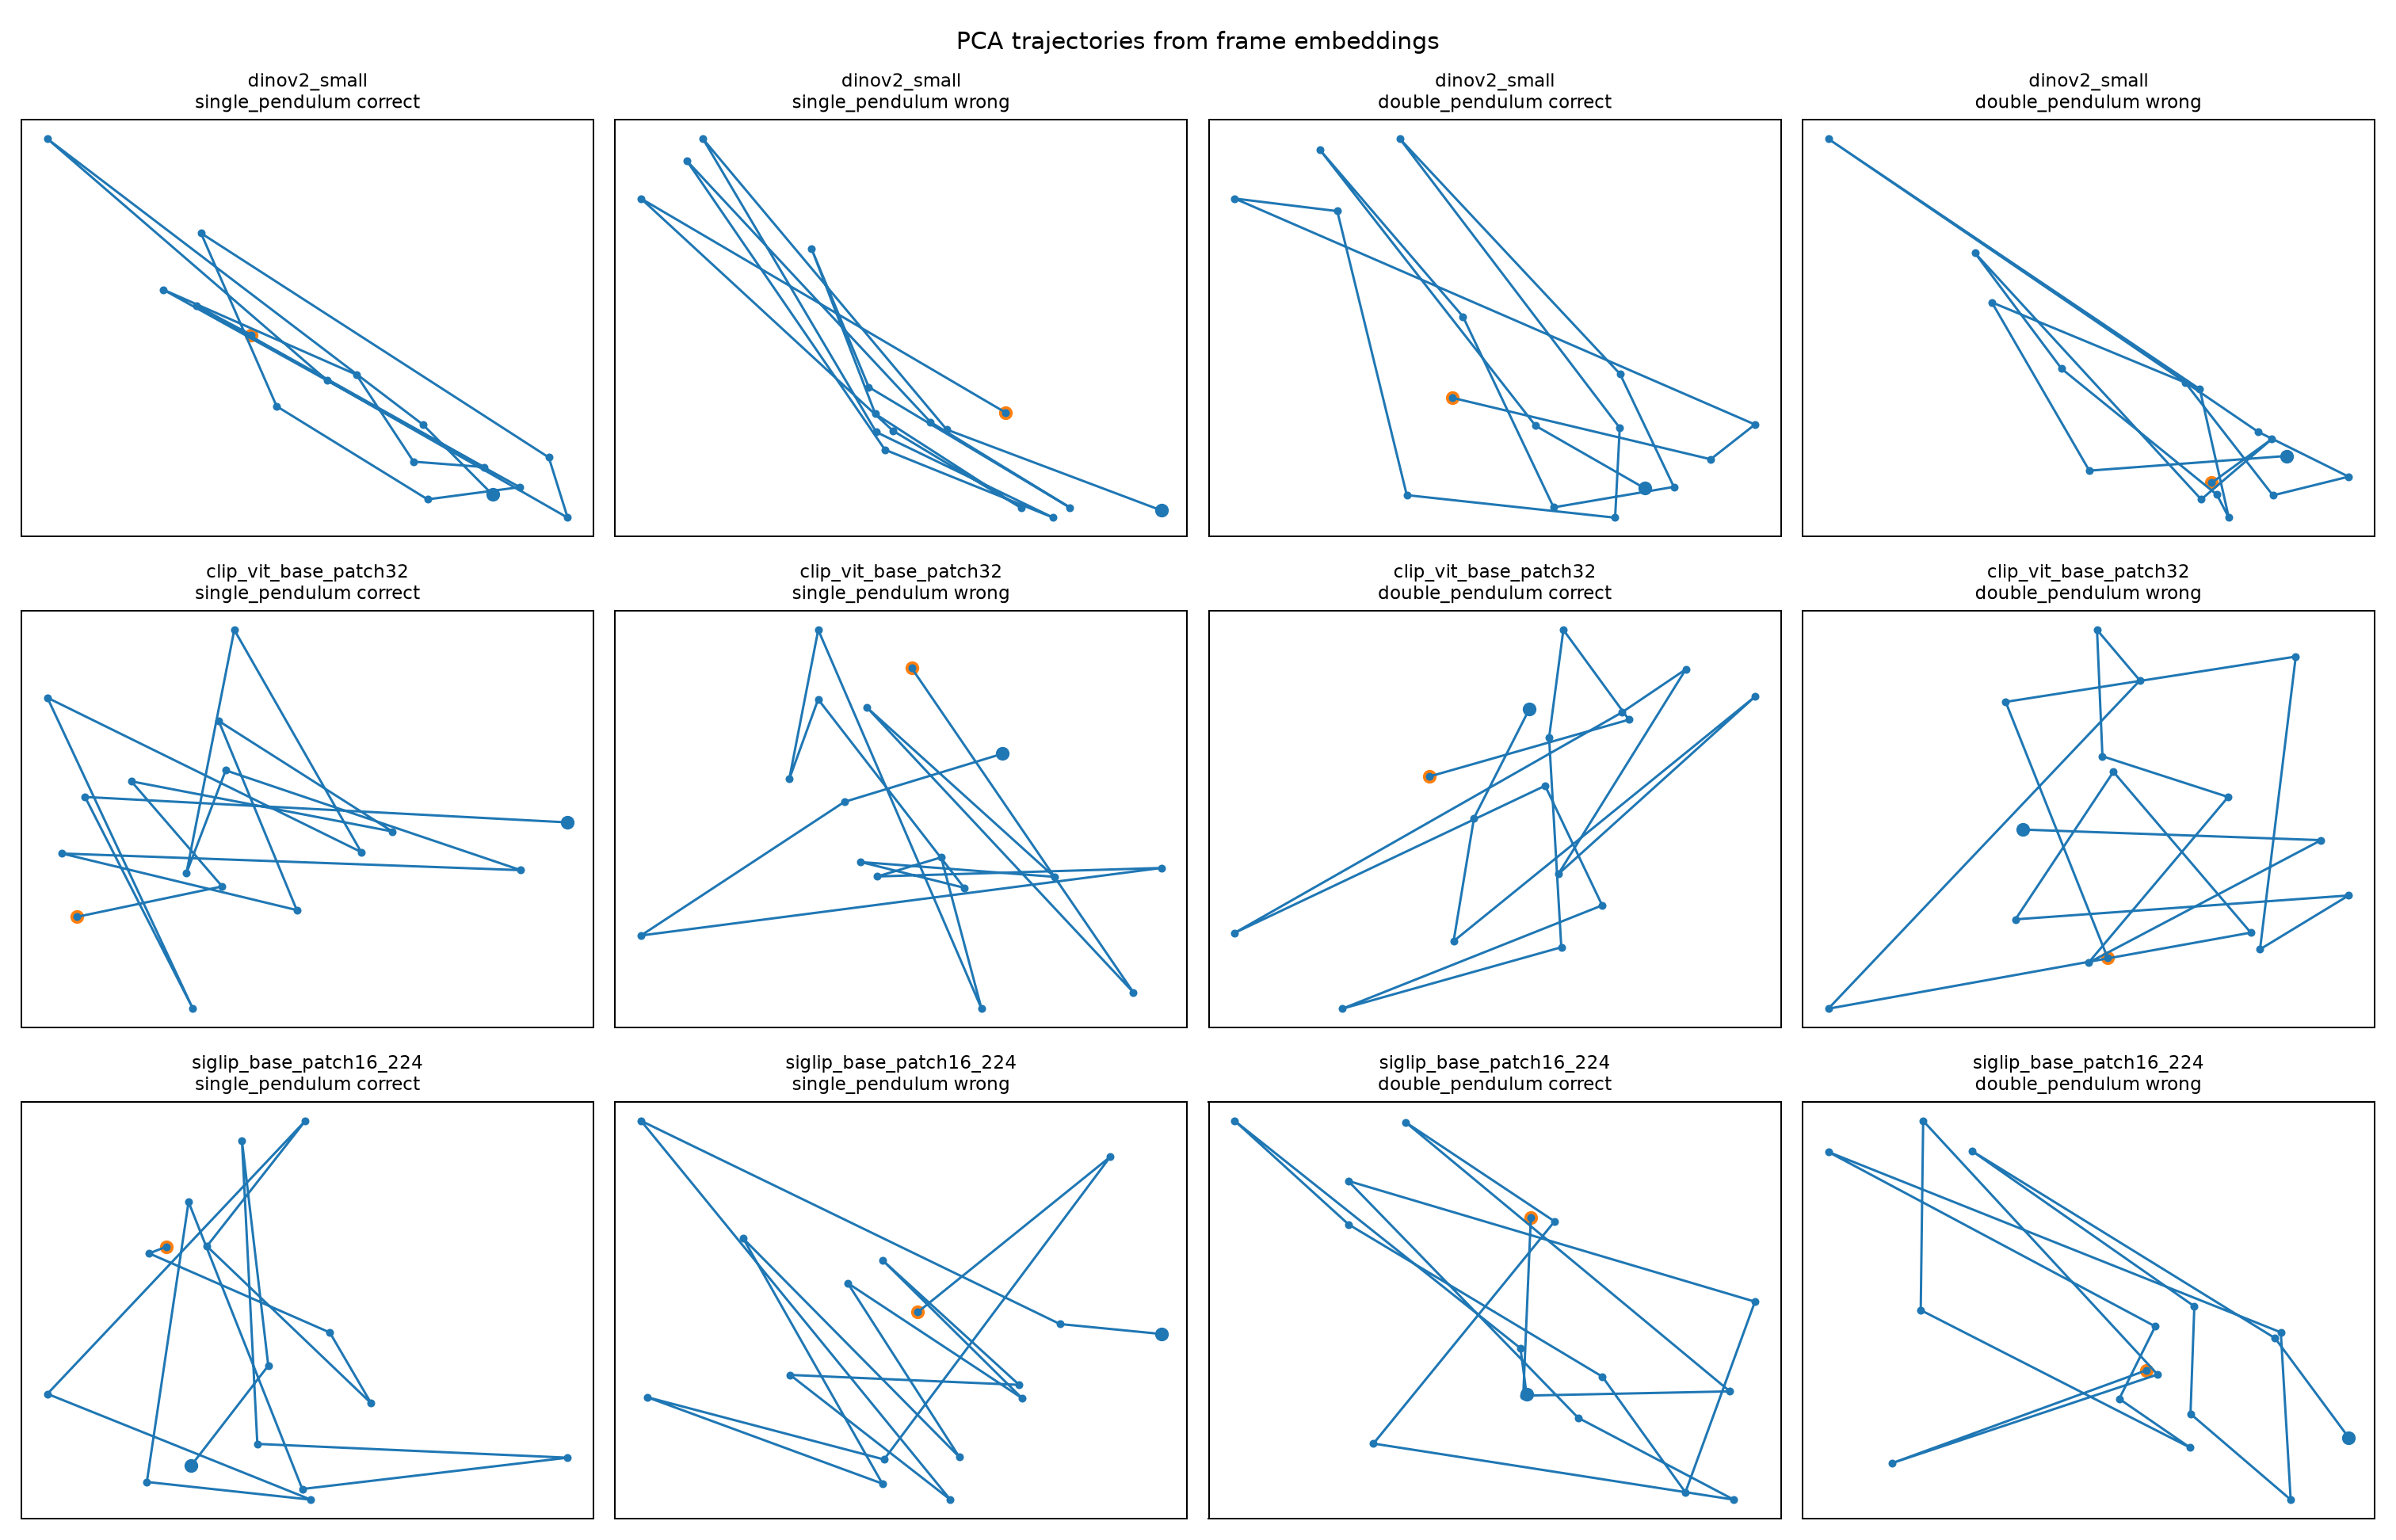
\includegraphics[width=\linewidth]{generated/simulated_pendulum/figures/pca_trajectories.png}
\caption{Qualitative PCA visualisation of selected latent trajectories. Each point is a sampled frame embedding. This figure is intended as an illustration of trajectory behaviour rather than the primary quantitative evidence.}
\label{fig:sim-pca-trajectories}
\end{figure}

\begin{figure}[t]
\centering
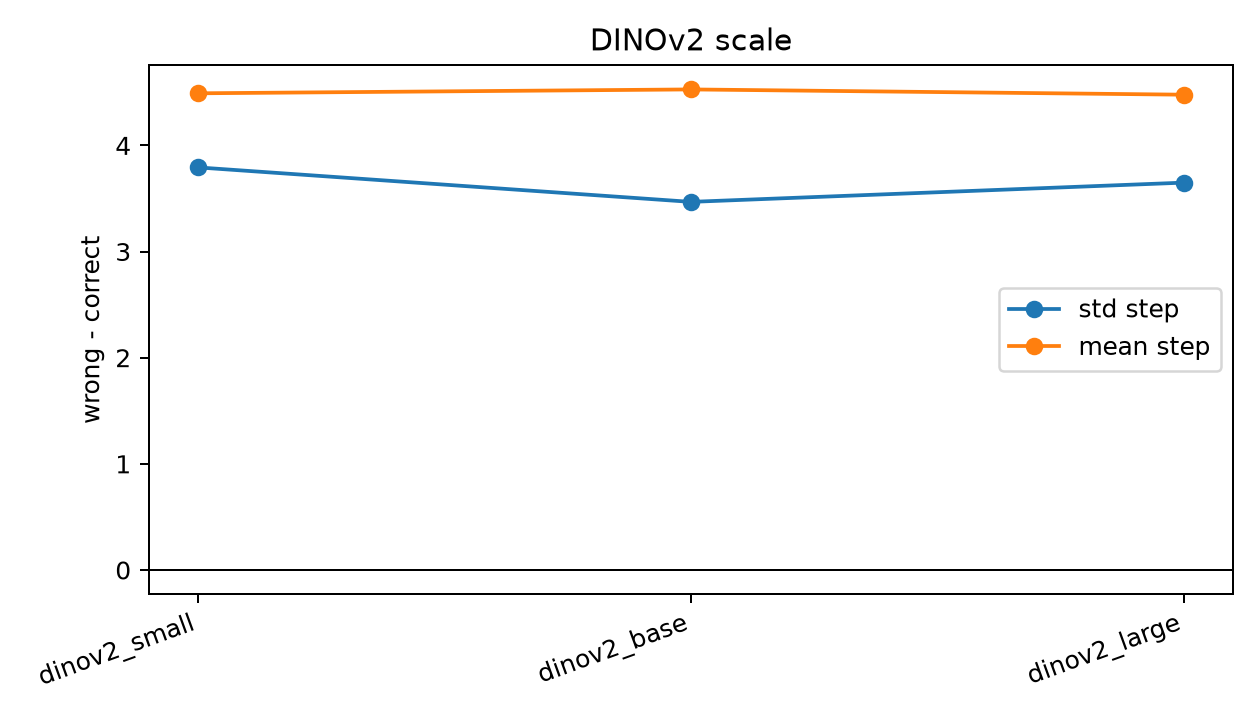
\includegraphics[width=0.48\linewidth]{generated/simulated_pendulum/figures/dinov2_scale.png}
\hfill
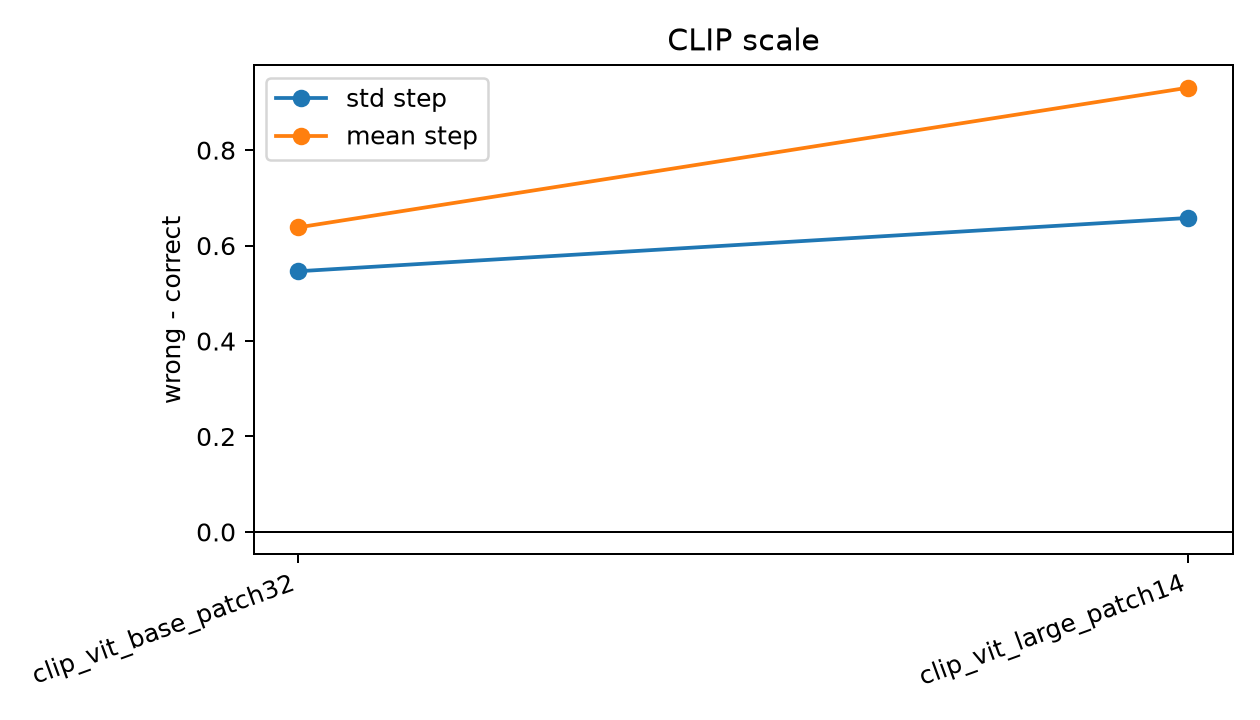
\includegraphics[width=0.48\linewidth]{generated/simulated_pendulum/figures/clip_scale.png}
\caption{Model-scale comparisons for DINOv2 and CLIP. DINOv2 models consistently show positive step-distance deltas, but the effect is not monotonic with scale. CLIP-B/32 is more separable than CLIP-L/14 in this benchmark.}
\label{fig:sim-scale-comparison}
\end{figure}


\subsection{Encoder Family And Scale}
DINOv2 models show the largest absolute step-distance changes. DINOv2-small,
DINOv2-base, and DINOv2-large all produce positive step-distance deltas, but the
effect does not increase monotonically with model size. DINOv2-base gives the
largest mean-step delta, while DINOv2-small gives the largest standard-deviation
delta.

DINOv2-base has the highest AUC for mean step distance in this benchmark
($0.802$), followed by CLIP-B/32 ($0.785$) and DINOv2-small ($0.769$). This
suggests that self-supervised visual representations are particularly sensitive
to the controlled pendulum perturbations, but the result is not simply a matter
of model size. SigLIP, Swin, and ViT also show positive step-distance deltas,
but the separation is smaller. MAE-B provides the weakest signal in this
setting.

\section{Discussion}
The controlled simulation results support the central hypothesis that latent
trajectories can reveal physically implausible motion. The clearest evidence is
not that wrong videos produce less straight trajectories, but that they produce
larger and less stable frame-to-frame latent movement. This distinction is
important. For periodic systems such as pendulums, a correct trajectory may
naturally loop or curve in representation space. Therefore, straightness alone
is too crude as a physics-consistency metric.

The encoder comparison also shows that the result is representation-dependent.
DINOv2 gives the largest absolute step-distance changes and the strongest AUC
for mean step distance in the current larger run. MAE performs poorly,
suggesting that not all pretrained image encoders are equally useful for
temporal physical diagnostics. A single universal score would hide these
differences, so the report should present model-specific behaviour.

The pairwise separation result makes the evidence stronger but also highlights
the current limitation. Correct-wrong pairs tend to be further apart than
correct-correct pairs, yet the distributions still overlap. This means the
latent trajectory signal is useful as a diagnostic measure, but it is not yet a
complete classifier for physical correctness. More simulated variants are
needed to estimate how robust the separation is across initial conditions,
wrong-physics types, and encoder families.

There are still limitations. The current benchmark is small, with only single-
and double-pendulum systems. The videos are visually simple, so the conclusions
may not transfer directly to natural videos or complex generated scenes. The
metrics are also computed from uniformly sampled frame embeddings, not from
explicit physical state estimates. They should therefore be interpreted as
diagnostic representation signals rather than direct measurements of physical
law violation.

% Auto-generated by generated_analysis/summarize_project_plan_results.py
\subsection{Connection To The Original Project Plan}
The original project plan proposed a small-scale framework for testing whether videos preserve basic physical regularities over time. The present work keeps this aim but introduces controlled simulation as the main source of ground-truth dynamics. This change was made because early AI-generated videos were useful for pipeline validation but did not provide reliable labels for physical correctness.

The resulting benchmark directly supports the embedding-based temporal analysis proposed in the plan. Correct and wrong pendulum dynamics are compared through latent trajectory metrics, pairwise trajectory separation, and selected patch-level feature and attention visualisations. Collision and occlusion/object permanence remain natural extensions for the final version of the benchmark.

\begin{figure}[htbp]
\centering
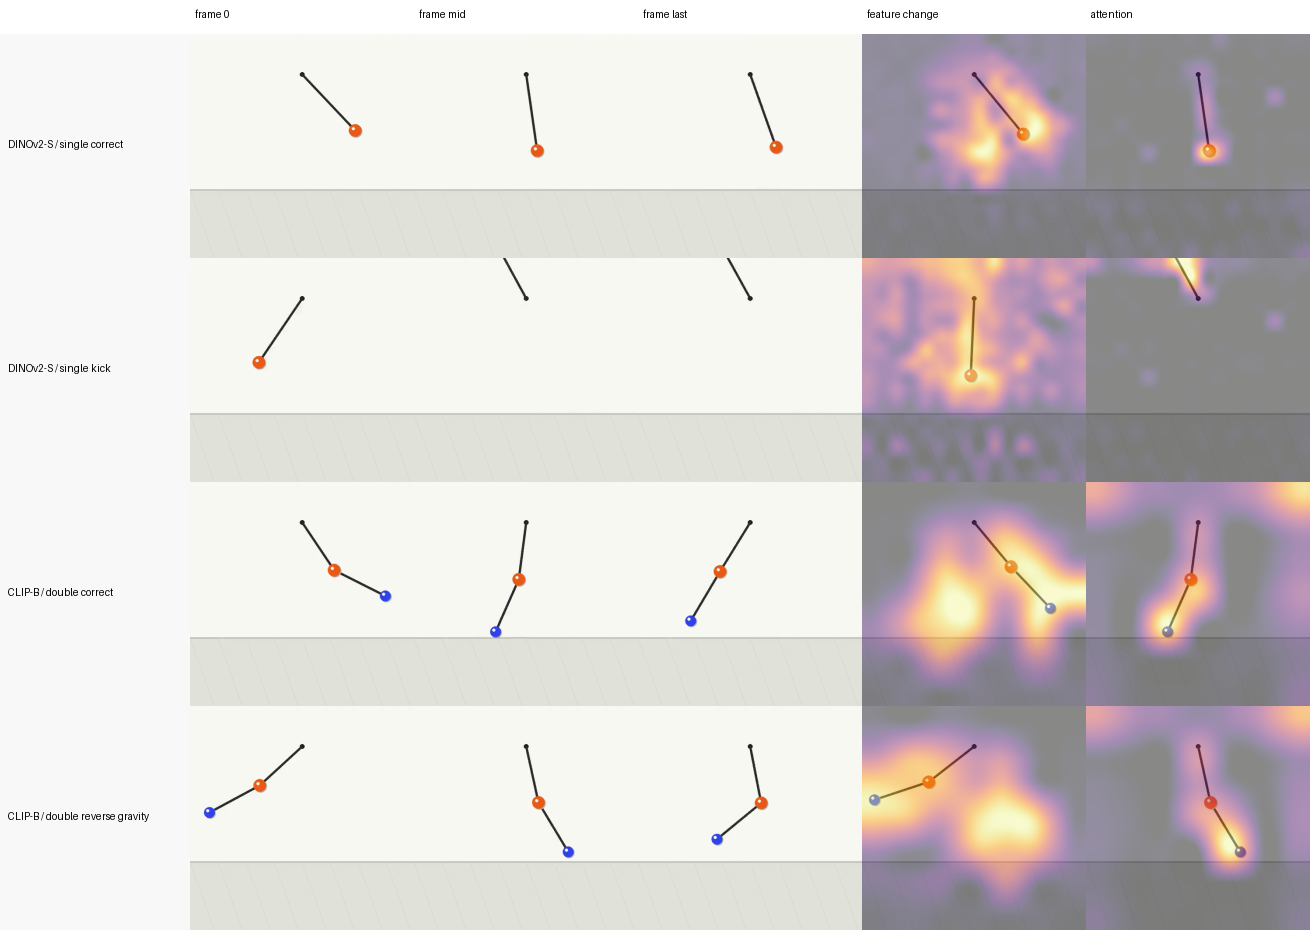
\includegraphics[width=\textwidth]{generated/simulated_pendulum/qualitative/qualitative_case_montage.png}
\caption{Selected qualitative case studies. Each row shows sampled frames, a patch feature-change map, and an attention overlay when available.}
\label{fig:qualitative-case-montage}
\end{figure}

\section{Conclusion}
This project developed and tested an evaluation pipeline for studying physical
consistency through visual latent trajectories. The move from AI-generated toy
videos to controlled simulated pendulum videos was essential: it allowed correct
and wrong physics labels to be defined explicitly rather than inferred from
imperfect prompts. On the simulated benchmark, wrong-physics videos generally
produce larger and more variable frame-to-frame latent movements. Step-distance
metrics are more reliable than straightness or curvature for this setting.

The results suggest that latent trajectory analysis is a useful diagnostic tool,
but not a complete physics evaluator. The most promising next direction is a
combined analysis of trajectory metrics, patch-level feature changes, and
attention maps across model families and model scales.

% References
\bibliographystyle{plain}
\bibliography{references}  % BibTeX references are saved in references.bib

\end{document}
